\documentclass[serif,xcolor=pdftex,dvipsnames,table,hyperref={bookmarks=false}]{beamer}

%%%%%%%%%%%%%%%%
% Change the macros below to configure the title slides
% for your course.
\newcommand{\coursename}{COMPSCI 589}
\newcommand{\instructor}{Benjamin M. Marlin}
\newcommand{\university}{University of Massachusetts Amherst}
\newcommand{\department}{College of Information and Computer Sciences}
%%%%%%%%%%%%%%%%


\newcommand{\settitlecard}[2]{
  \title[\coursename  Lecture #1] 
    {\coursename \\ Lecture #1: #2}
     \author[\instructor]{\instructor}
     \institute[\university]{
     \department\\
     \university
   }
\date{}
}

\newcommand{\maketitlepage}{
  \begin{frame}
  \titlepage
  \center{
    %If you use the slides unmodified, retain the attribution below
    \tiny{Slides by Benjamin M. Marlin (marlin@cs.umass.edu). \\
    \vspace{-1em}Created with support from National Science Foundation Award\# IIS-1350522. 
    %If you modify the slides, please retain the alternate attribution below
    %\tiny{Based on slides by Benjamin M. Marlin (marlin@cs.umass.edu). \\    
    %\vspace{-1em}Created with support from National Science Foundation Award\# IIS-1350522. 
    }                                              
  }  
  \end{frame}
}

\AtBeginSection[]
{
  \begin{frame}<beamer>{Outline}
    \tableofcontents[currentsection,subsectionstyle=hide]
  \end{frame}
}


\newcommand{\cut}[1]{}

\newcommand{\iconbox}[4]{
  \only<#1-#2>{
    \begin{columns}[T]
      \column{0.5in}
           \includegraphics[width=0.5in]{#3}
       \column{3.7in}
            #4
    \end{columns}
    \medskip
    \medskip
    \medskip
  }
}

\mode<presentation>{
  \usepackage{../beamertheme589theme}
  \setbeamercovered{invisible}
}

\mode<handout>{
  \usepackage{../beamertheme589theme}
  \setbeamercovered{transparent}
}


\usepackage[english]{babel}
\usepackage[latin1]{inputenc}
\usepackage{times}
\usepackage[T1]{fontenc}
\usepackage{amsmath}
\usepackage{amssymb}
\usepackage[noend]{algorithmic}
\usepackage{algorithm}
\usepackage{listings}

\renewcommand\mathfamilydefault{\rmdefault}

\newcommand{\setA}{\mathcal{A}}
\newcommand{\setB}{\mathcal{B}}
\newcommand{\setS}{\mathcal{S}}
\newcommand{\setV}{\mathcal{V}}
\DeclareMathOperator*{\union}{\bigcup}
\DeclareMathOperator*{\intersection}{\bigcap}
\DeclareMathOperator*{\Val}{Val}
\newcommand{\mbf}[1]{{\mathbf{#1}}}
\DeclareMathOperator*{\argmax}{arg\,max}
\DeclareMathOperator*{\argmin}{arg\,min}
\DeclareMathOperator*{\sign}{sign}
\newcommand{\deriv}[2]{\frac{\partial{#1}}{\partial{#2}}}


\settitlecard{2}{KNN and Decision Trees}

\begin{document}

\maketitlepage

\section{Review}
\subsection{Foo}


\begin{frame}[t]{Views on Machine Learning}

\iconbox{1}{}{../Figures/mitchell.jpg}{\textbf{Mitchell (1997):} ``A computer program is said to learn from experience E with respect to some class of tasks T and performance measure P, if its performance at tasks in T, as measured by P, improves with experience E.''\\[12pt]  Substitute ``training data D'' for  ``experience E.''}

\end{frame}

\begin{frame}[t]{Machine Learning Tasks}
 \centering
 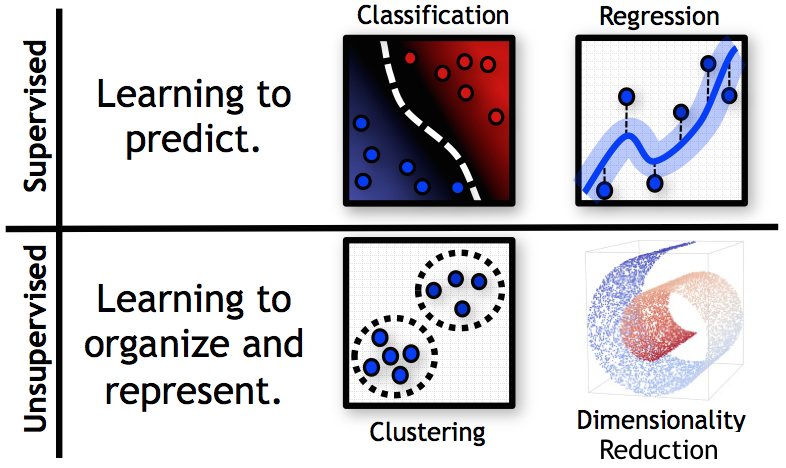
\includegraphics[width=4in]{../Figures/learning_problems.png}
\end{frame}

\begin{frame}[t]{Machine Learning Approaches}
  \begin{itemize}
    \item \textbf{Non-Parametric:} Learning is accomplished by storing the training data (memorization).
    
    \item \textbf{Parametric:} Learning is accomplished by using an algorithm to adapt the parameters in a mathematical or statistical model given training data. For exmaple:\\
    
    
  \end{itemize}
\end{frame}


\section{Classification}
\subsection{Foo}

\begin{frame}[t]{The Classification Task}

\begin{block}{Definition: The Classification Task}
Given a feature vector $\mbf{x}\in\mathbb{R}^D$ that describes an object that belongs to one of $C$ classes from the set $\mathcal{Y}$, predict which class the object belongs to.
\end{block}

\end{frame}

\begin{frame}[t]{Example: Digits}
 \centering
 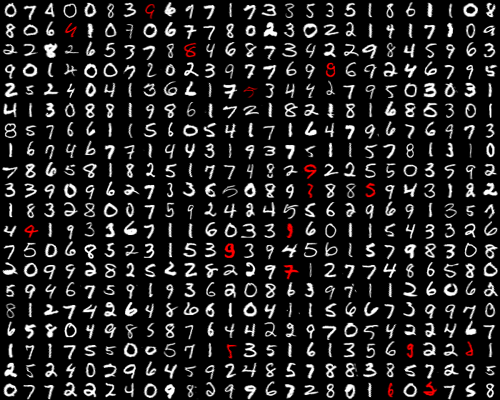
\includegraphics[width=3.5in]{../Figures/mnist.png}
\end{frame}

\begin{frame}[t]{Example: Natural Images}
 \centering
 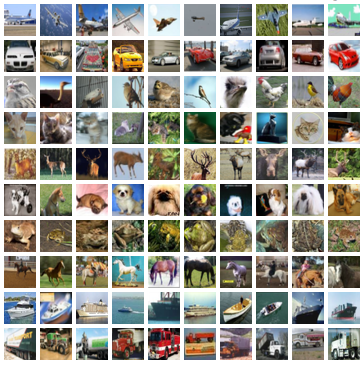
\includegraphics[width=3.5in]{../Figures/cifar.png}
\end{frame}

\begin{frame}[t]{Example: Synthetic Images}
 \centering
 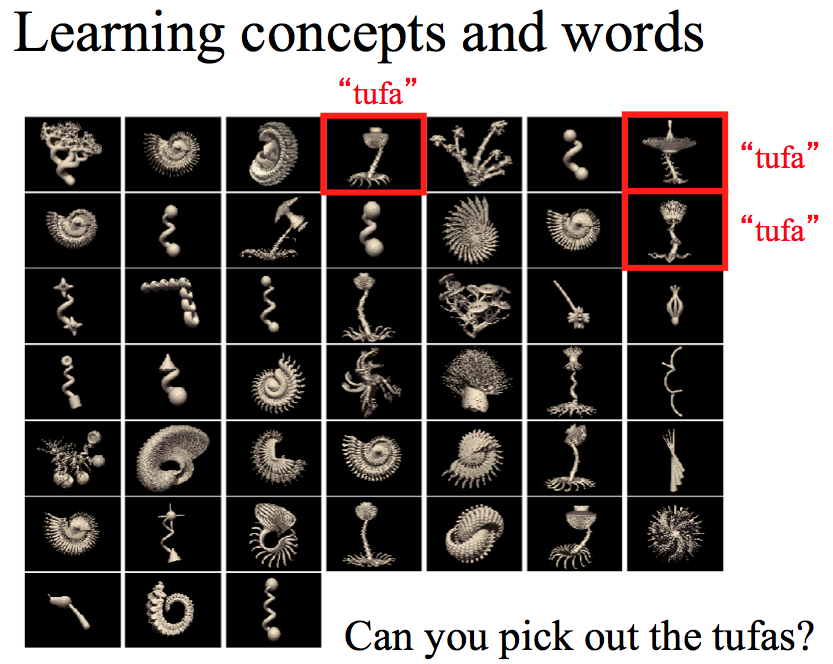
\includegraphics[width=3.5in]{../Figures/tufas.png}
\end{frame}

\begin{frame}[t]{The Classifier Learning Problem}
\begin{block}{Definition: Classifier Learning}
Given a data set of example pairs $\mathcal{D}=\{(\mbf{x}_i,y_i),i=1:N\}$ where $\mbf{x}_i\in\mathbb{R}^D$ is a feature vector and $y_i\in \mathcal{Y}$ is a class label, learn a function $f:\mathbb{R}^D\rightarrow \mathcal{Y}$ that accurately predicts the class label $y$ for any feature vector $\mbf{x}$.
\end{block}
\end{frame}

\begin{frame}[t]{Classification Error and Accuracy}

\begin{block}{Definition: Classification Error Rate}
Given a data set of example pairs $\mathcal{D}=\{(\mbf{x}_i,y_i),i=1:N\}$ and a function $f:\mathbb{R}^D\rightarrow \mathcal{Y}$, the classification error rate of $f$ on $\mathcal{D}$ is:
$$Err(f,\mathcal{D}) = \frac{1}{N}\sum_{i=1}^N\mathbb{I}(y_i \neq f(\mbf{x}_i))$$
\end{block}

\pause
\begin{block}{Definition: Classification Accuracy Rate}
Given a data set of example pairs $\mathcal{D}=\{(\mbf{x}_i,y_i),i=1:N\}$ and a function $f:\mathbb{R}^D\rightarrow \mathcal{Y}$, the classification accuracy rate of $f$ on $\mathcal{D}$ is:
$$Acc(f,\mathcal{D}) = \frac{1}{N}\sum_{i=1}^N\mathbb{I}(y_i = f(\mbf{x}_i))$$
\end{block}


\end{frame}


\section{KNN}
\subsection{Foo}
\begin{frame}[t]{K Nearest Neighbors Classification}

The KNN classifier is a non-parametric classifier that simply stores the training data $\mathcal{D}$
and classifies each new instance $\mbf{x}$ using a majority vote over its' set of $K$ nearest neighbors $\mathcal{N}_K(\mbf{x})$ computed using any distance function $d:\mathbb{R}^D \times\mathbb{R}^D \rightarrow \mathbb{R} $.

\pause
\begin{block}{KNN Classification Function}
$$f_{KNN}(\mbf{x}) = \argmax_{y\in\mathcal{Y}} \sum_{i\in \mathcal{N}_K(\mbf{x})} \mathbb{I}[y_i=y]$$
\end{block}

\pause Use of KNN requires choosing the distance function $d$ and the number of neighbors $K$.

\end{frame}

\begin{frame}[t]{Distance and Similarity}

\begin{itemize}
\item In general, KNN can work with any distance function $d$ satisfying non-negativity $d(\mbf{x},\mbf{x}')\geq 0$ and identity of indiscernibles $d(\mbf{x},\mbf{x})=0$.

\pause\item Alternatively, KNN can work with any similarity function $s$ satisfying non-negativity $s(\mbf{x},\mbf{y})\geq 0$ that attains it's maximum on indiscernibles $s(\mbf{x},\mbf{x})=\max_{\mbf{x}'} s(\mbf{x},\mbf{x}')$.

\pause\item However, the more structure the distance or similarity function has  (symmetry, triangle inequality), 
the more structure you can exploit when designing algorithms.

\end{itemize}

\end{frame}

\begin{frame}[t]{Distance Metrics}

\begin{block}{Definition: Minkowski Distance ($\ell_p$ norms)}
Given two data vectors $\mbf{x},\mbf{x}' \in \mathbb{R}^D$, the Minkowski Distance with parameter $p$ (the $\ell_p$ norm) is a proper metric defined as follows:

\begin{align*}
d_p(\mbf{x},\mbf{x}') &=  ||\mbf{x}-\mbf{x}'||_p \\
&=\left(\sum_{i=1}^D |x_d-x'_d|^p\right)^{1/p}
\end{align*}
\end{block}
\pause Special cases include Euclidean distance ($p=2$), Manhattan distance ($p=1$) and Chebyshev distance ($p=\infty$).

\end{frame}

\begin{frame}[t]{Brute Force KNN}

\begin{itemize}
\item Given any distance function $d$, brute force KNN works by computing the distance $d_i = d(\mbf{x}_i,\mbf{x}_*)$ from a target point $\mbf{x}_*$ to all of the training points $\mbf{x}_i$.

\pause \item You then simply sort the distances $\{d_i,i=1:N\}$ and choose the data cases with the $K$ smallest distances to form the neighbor set $\mathcal{N}_K(\mbf{x}_*)$. Using a similarity function is identical, but you select the $K$ most similar data cases. 

\pause \item Once the $K$ neighbors are selected, applying the classification rule is easy.
\end{itemize}

\end{frame}

\begin{frame}[t]{KNN Variants}

\begin{itemize}
\item Instead of giving all of the $K$ neighbors equal weight in the majority vote, a distance-weighted majority can be used:

\begin{align*}
f_{KNN}(\mbf{x}) &= \argmax_{y\in\mathcal{Y}} \frac{\sum_{i\in \mathcal{N}_K(\mbf{x})} w_i \mathbb{I}[y_i=y]}
{\sum_{i\in \mathcal{N}_K(\mbf{x})} w_i}\\
w_i &= \exp(-\alpha d_i)
\end{align*}

\pause
\item Instead of a brute force nearest neighbor search, data structures like ball trees can be constructed over the training data that support nearest neighbor search with lower amortized computational complexity.

\end{itemize}

\end{frame}

\begin{frame}[t]{KNN Trade-Offs}

\begin{itemize}
\item Low bias: Converges to the correct decision surface as data goes to infinity.

\pause \item High variance: Lots of variability in the decision surface when amount of data is low.

\pause \item Curse of dimensionality: Everything is far from everything else in high dimensions.

\pause \item Space and Time Complexity: Need to store all training data and perform neighbor search can make the method
use a lot of memory and take a lot of time.
\end{itemize}

\end{frame}

\section{Decision Trees}
\subsection{foo}

\begin{frame}[t]{Decision Tree}

\begin{itemize}
\item A classical decision tree classifies data cases using a conjunction of rules organized into a binary tree structure.

\pause\item Each internal node in a classical decision tree contains a rule of the form $(x_d<t)$ or $(x_d=t$) that tests a single data dimension $d$ against a single value $t$ and assigns the data case to it's left or right sub-tree according to the result.

\pause \item A data case is routed through the tree from the root to a leaf. Each leaf node is associated with a class, and a data case is assigned the class of the leaf node it is routed to.

\end{itemize}

\end{frame}

\begin{frame}[t]{Example: Decision Tree for Flu}
 \centering
 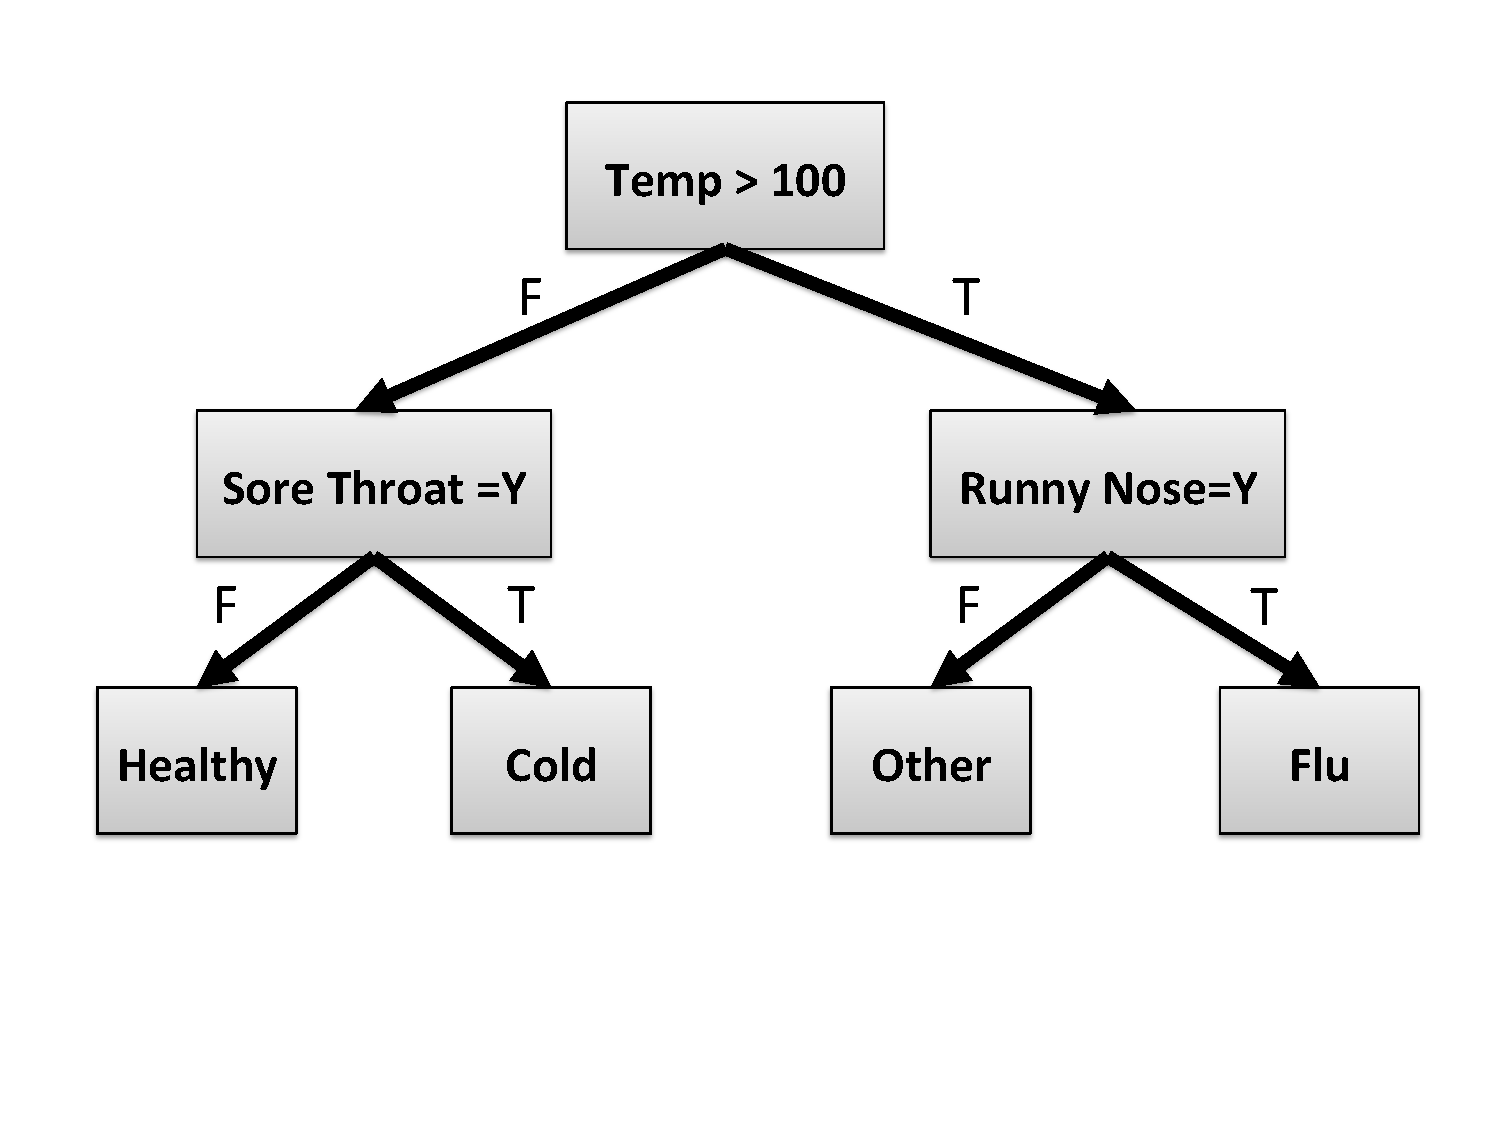
\includegraphics[width=4in]{../Figures/decision-tree.pdf}
\end{frame}

\begin{frame}[t]{Decision Tree Learning Algorithm}

\begin{itemize}
\item Decision trees are learned using recursive greedy algorithms that 
select the variable and threshold at each node from top to bottom.

\pause\item The learning algorithm begins with all data cases at the root of the tree.

\pause\item The algorithm selects a variable and a threshold to split on according to a heuristic.

\pause\item The algorithm applies the chosen rule and assigns each data case to
the left or right sub-tree.

\pause\item The algorithm then recurses on the child nodes until a given stopping condition is satisfied.

\pause\item When the stopping condition is satisfied, the current node is a leaf
in the tree. It is typically assigned a label that corresponds to the most common label of the
data cases it contains.

\cut{
The two main criteria used to evaluate the the split that results from 
a potential variable $d$ and threshold $t$ are Gini Impurity ($C_{GI}$) and information gain ($C_{IG}$).

\pause\item Suppose a given variable $d$ and threshold $t$ result in a distribution of class labels in the proportions
$p_1,p_2,...,p_C$ for the $C$ classes.

\pause
$$
C_{GI} = \sum_{c=1}^C p_i(1-p_i)\;\;\;\;\;\;
C_{IG} = -\sum_{c=1}^C p_i \log(p_i)
$$

\pause\item The decision tree construction algorithm recursively searches for optimal (variable, threshold) pairs according
to a given criteria down to a specified depth.
}
\end{itemize}

\end{frame}


\begin{frame}[t]{Decision Tree Learning}

\begin{itemize}
\item The main stopping criteria used are all data cases assigned to a node have the same label, the number of data cases assigned to the node falls below a threshold, and the node is at the maximum allowable depth.

\pause\item Given sufficient depth, a decision tree can approximate any classification function to arbitrary accuracy.

\pause\item There are a number of heuristics for selecting variables and thresholds to split on.
In general, these heuristics are aimed at producing splits of the training data that are as homogeneous as possible in terms of the labels.
\end{itemize}

\end{frame}

\begin{frame}[t]{Decision Tree Trade-Offs}

\begin{itemize}
\item Interpretability: The learned model is easy to understand as a collection of rules.

\pause \item Test Complexity: Shallow trees can be extremely fast classifiers at test time.

\pause \item Train Complexity: Finding optimal trees is NP-complete, thus need for greedy heuristics.

\pause \item Representation: Splitting on single variables can require very large trees to
accurately model non-axis aligned decision boundaries.
\end{itemize}

\end{frame}




\end{document}
